This algorithm is a step towards a more complex control algorithm. Some minor logic replaces the random generator in the previous solution. 

\begin{algorithm}[H]
  \If{More than 1 balloon at current space}{
  Calculate projections\;
  
 	\If{optionUp < optionDown} 
 	{Go up}
 	\Else
 	{Go down}

 }
 \Else
 {Stay in current layer}
 \caption{Control Algorithm 2}
 \label{alg2}
\end{algorithm}

The balloon fetches the wind vectors from neighbouring wind layers and uses them to weigh its options. It computes the number of balloons occupying three different cells:
\begin{enumerate}
\item The cell to which the balloon's current wind layer will move it.
\item The cell to which the the wind layer above the balloon's current wind layer would move it.
\item The cell to which the the wind layer below the balloon's current wind layer would move it.
\end{enumerate}

The algorithm then determines which option has the cell with the lowest number of balloons and chooses that direction.
\begin{figure}
\centering
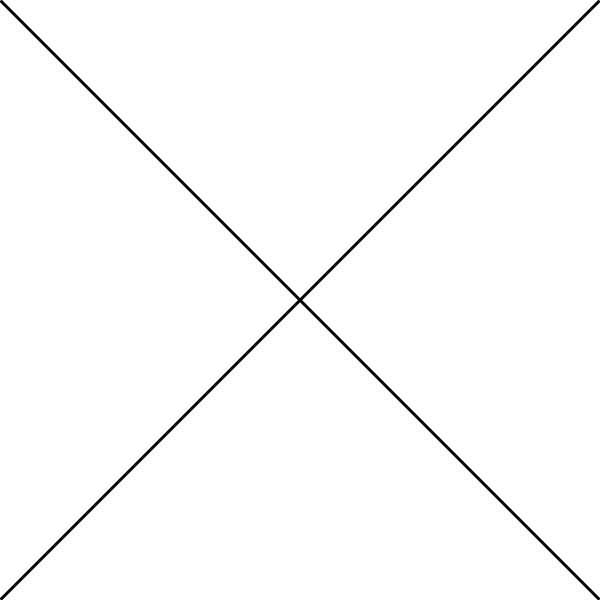
\includegraphics[scale=0.2]{graphics/todo.png}
\caption{Calculate projections}
\label{fig:projections}
\end{figure}

\begin{figure}
\centering
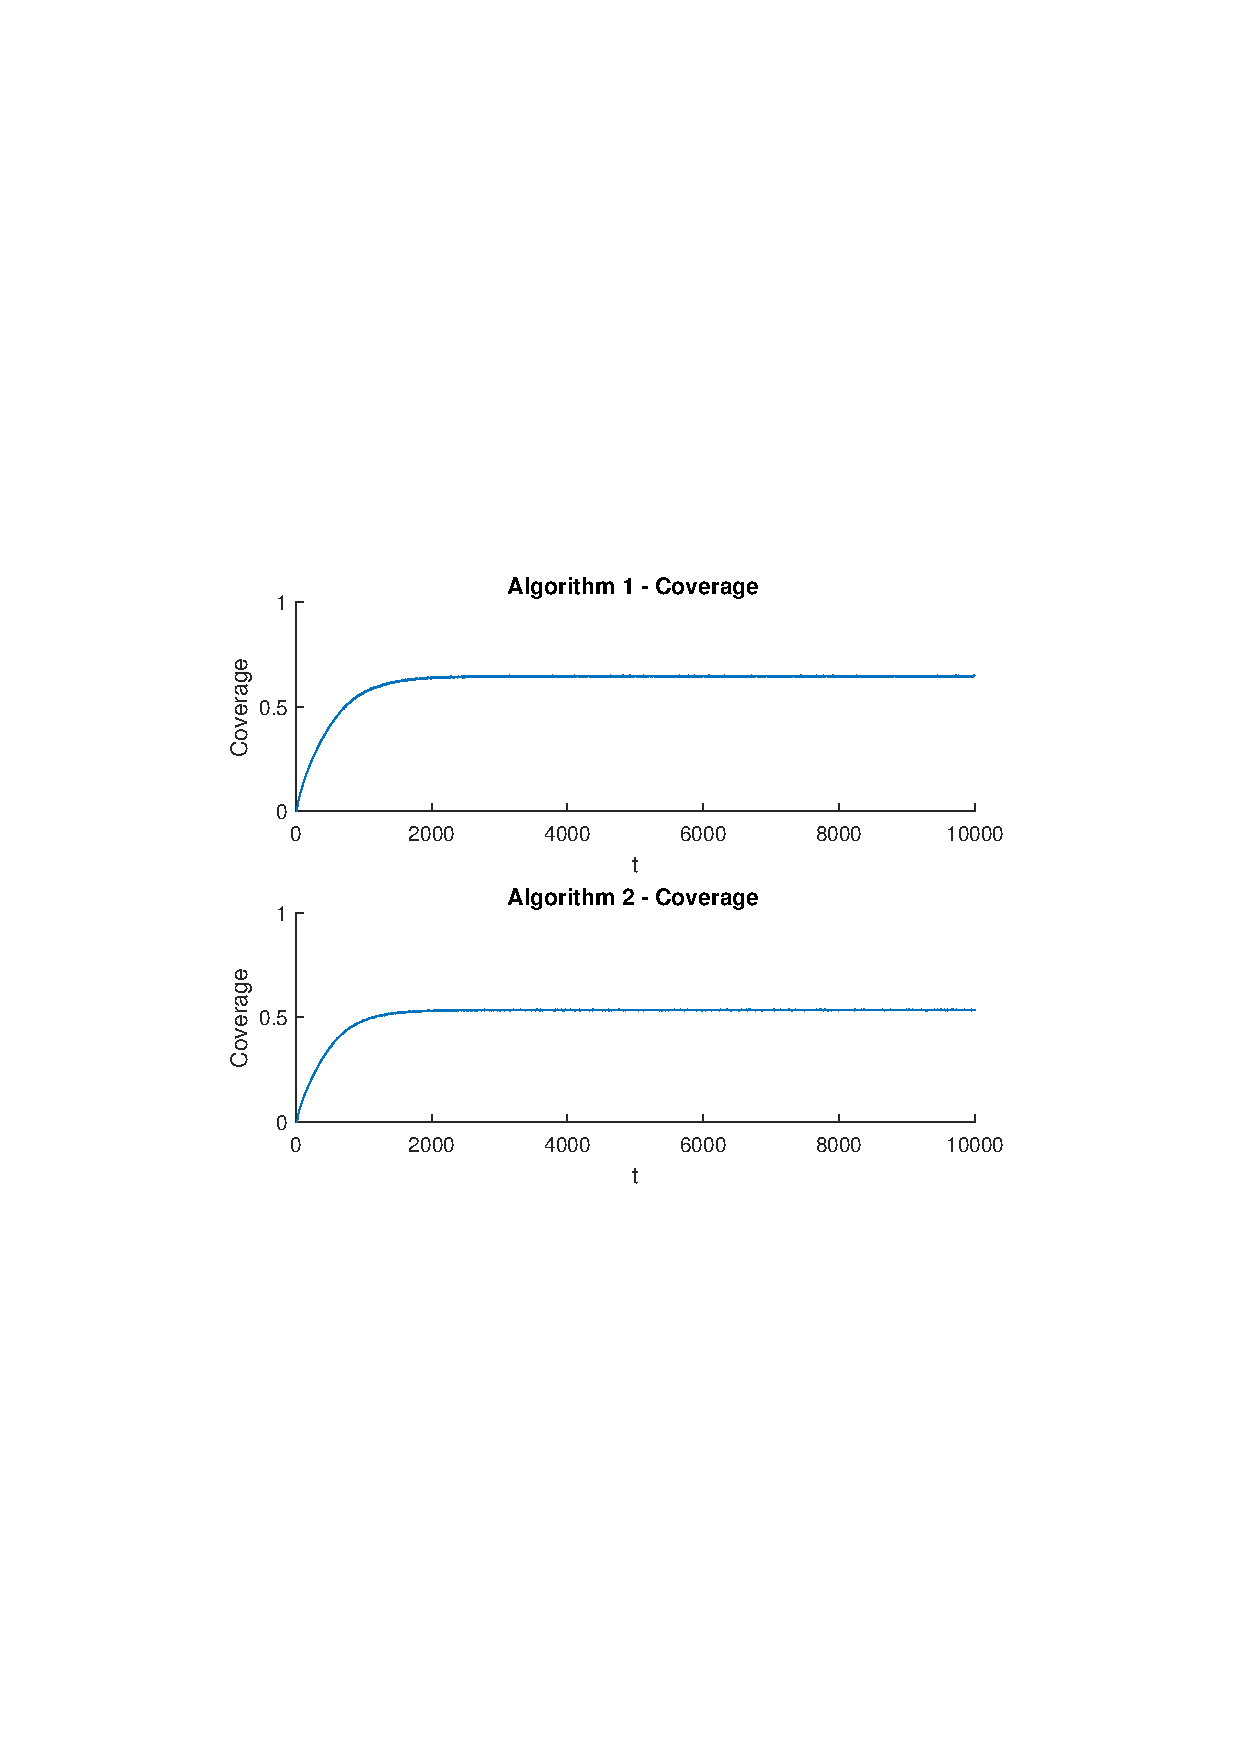
\includegraphics[width=\textwidth, trim={3cm 10cm 4cm 9cm},clip]{graphics/coverage_alg1_vs_alg2.pdf}
\caption{Algorithm 1 outperforms Algorithm 2}
\label{fig:alg1vsalg2}
\end{figure}
It is interesting to see that Algorithm 1 outperforms Algorithm 2 when it comes to coverage. Algorithm 1 reaches higher coverage like Figure \ref{fig:alg1vsalg2} clearly shows.